\chapter{Выполнение}

\section{Выбор языка программирования}
Для выполнения домашнего задания был выбран язык \texttt{C++}.

\section{Код программы}

Код программы приведен в листинге \ref{lst:code}.

\lstinputlisting[label=lst:code, caption=Реализация алгоритма поиска подстроки, firstline=4,lastline=23]{../src/main.cpp}

\chapter{Графовые модели программы}

\section{Граф управления}

На рисунке \ref{fg:mg} представлен граф управления.

\begin{figure}[h]
	\centering
	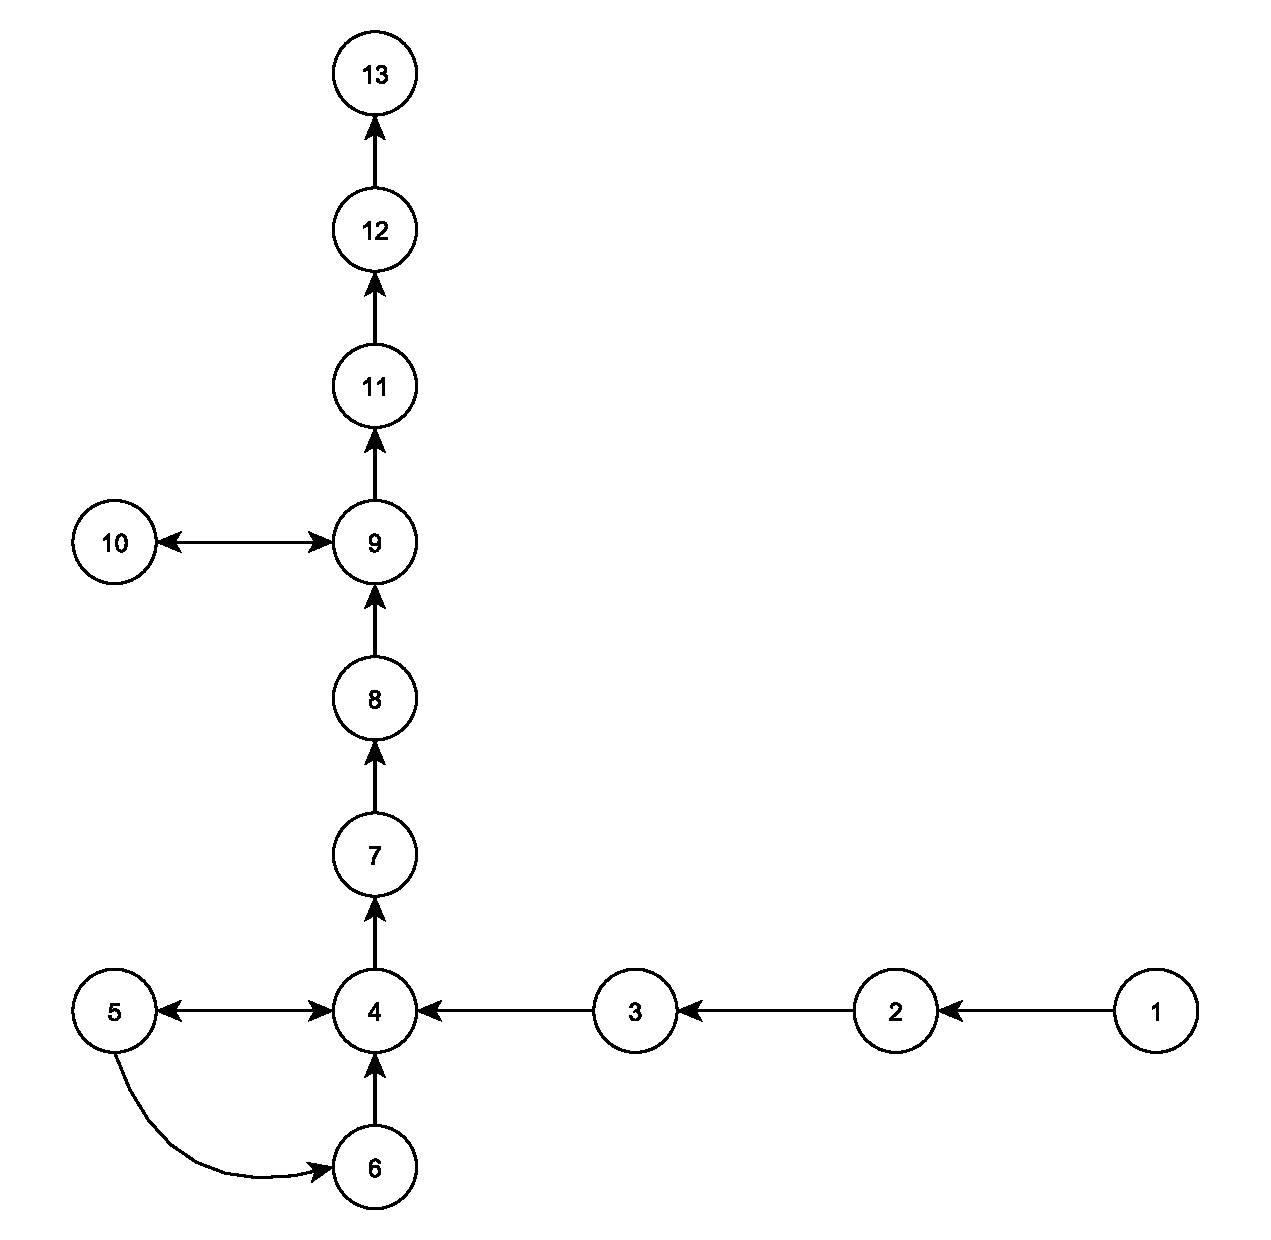
\includegraphics[height=0.6\textheight]{images/ГУ.pdf}
	\caption{Граф управления}
	\label{fg:mg}
\end{figure}

\clearpage

\section{Информационный граф}

На рисунке \ref{fg:ig} представлен информационный граф.

\begin{figure}[h]
	\centering
	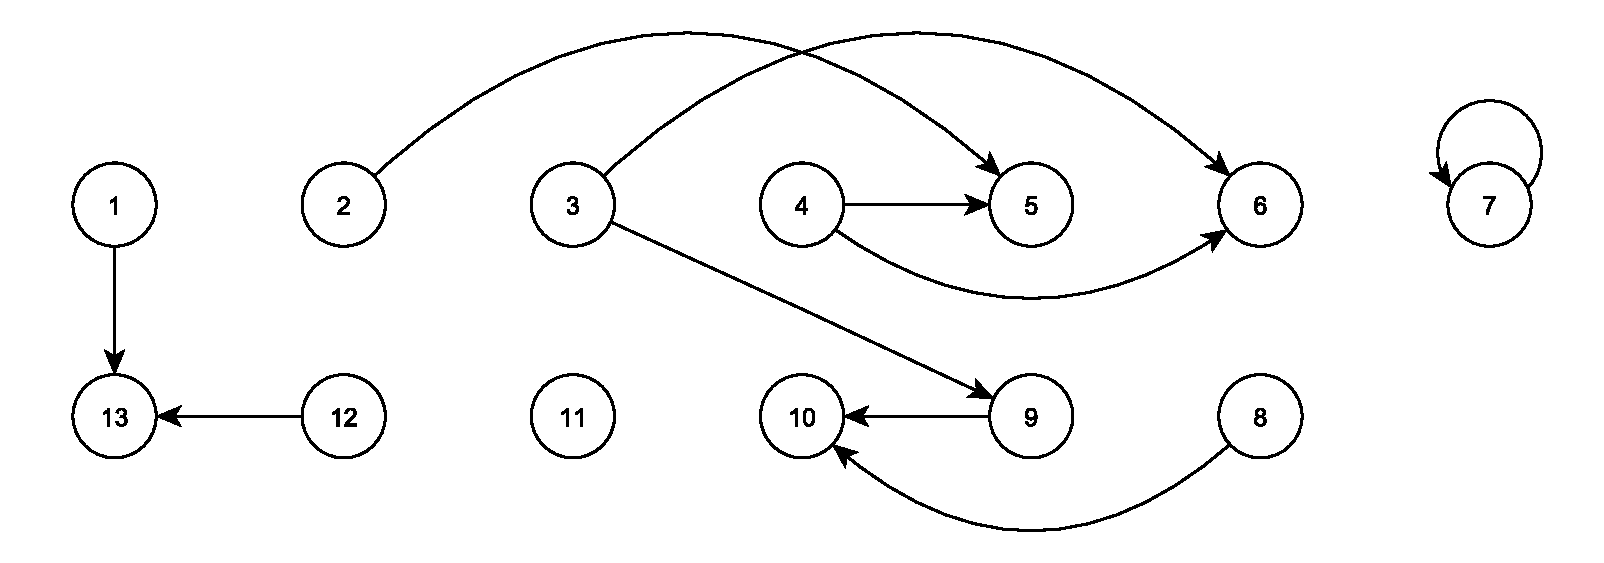
\includegraphics[height=0.23\textheight]{images/ИГ.pdf}
	\caption{Информационный граф}
	\label{fg:ig}
\end{figure}

Вершина 7 представляет собой операцию блокировки мьютекса, т.к. файл, куда записываются индексы вхождения подстроки --- критическая секция.
В информационном графе она связана сама с собой, т.к. операция блокировки мьютекса обращается к этому же мьютексу для проверки его состояния.

Вершина 11 представляет собой установку i-го бинарного семафора массива, который идентифицирует завершение выполнения функции.
В графе \ref{fg:ig} она не связана с другими вершинами потому что используется в управляющем потоке для отслеживания завершения работы каждого потока.

\clearpage

\section{Операционная история}

На рисунке \ref{fg:oi} представлена операционная история файла, содержащего $n$ символов и $m$ вхождений подстроки. 

\begin{figure}[h]
	\centering
	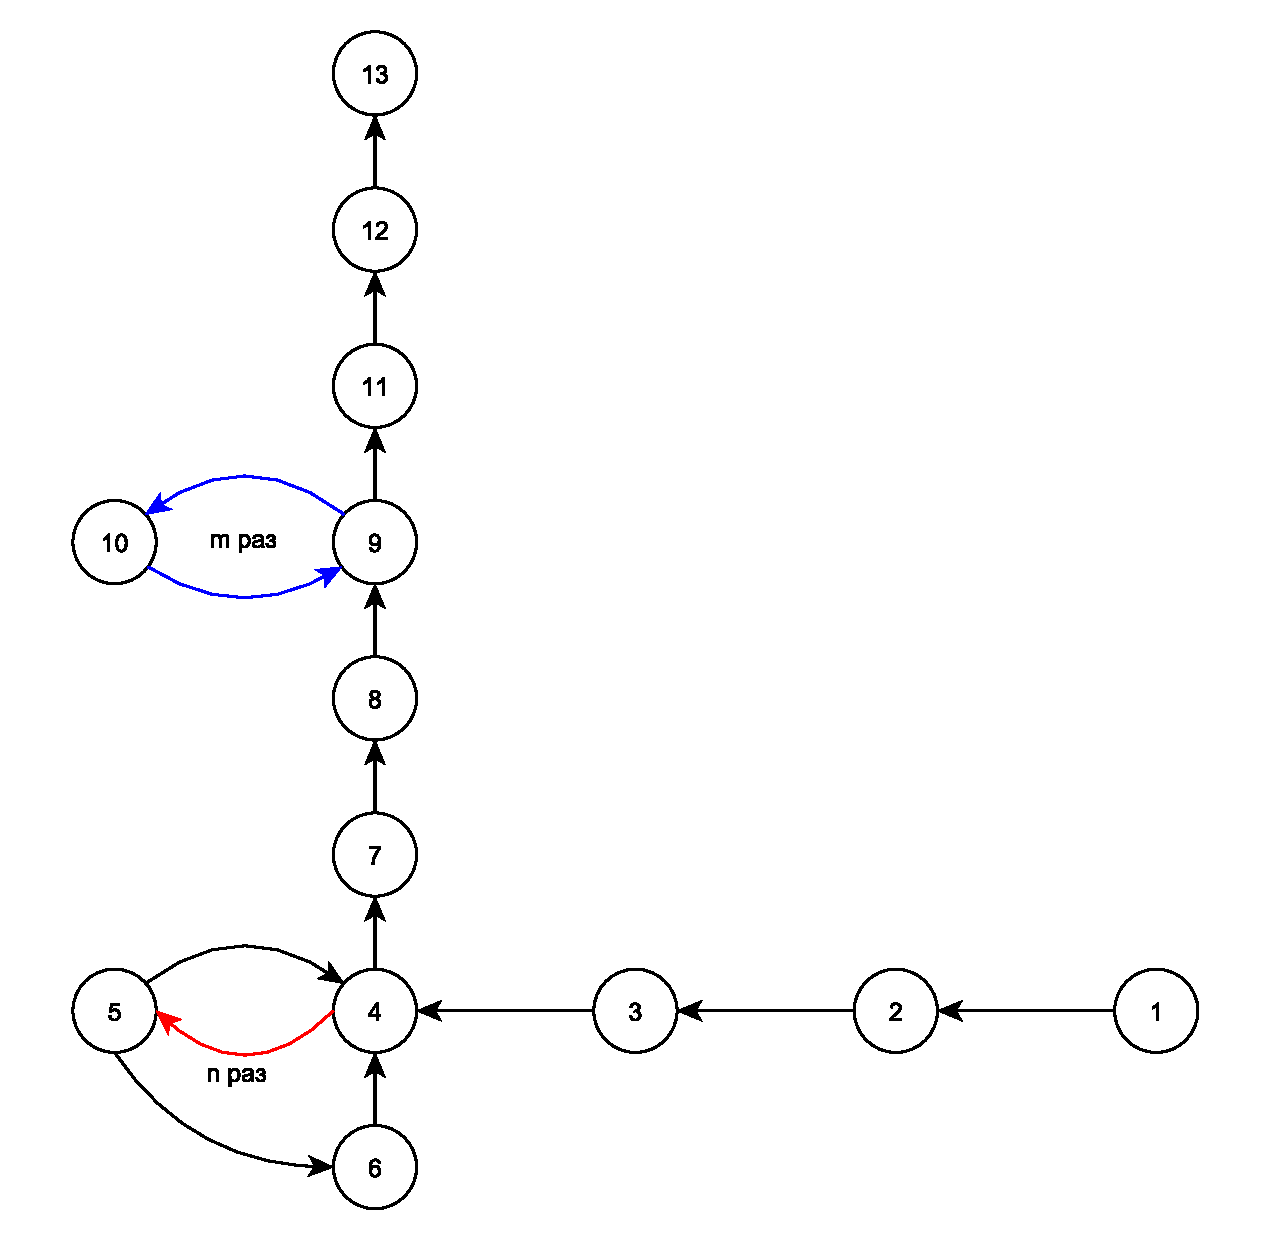
\includegraphics[height=0.6\textheight]{images/ОИ.pdf}
	\caption{Операционная история}
	\label{fg:oi}
\end{figure}

\clearpage

\section{Информационная история}

На рисунке \ref{fg:ii} представлена информационная история файла, содержащего $n$ и $m$ вхождений подстроки. 

\begin{figure}[h]
	\centering
	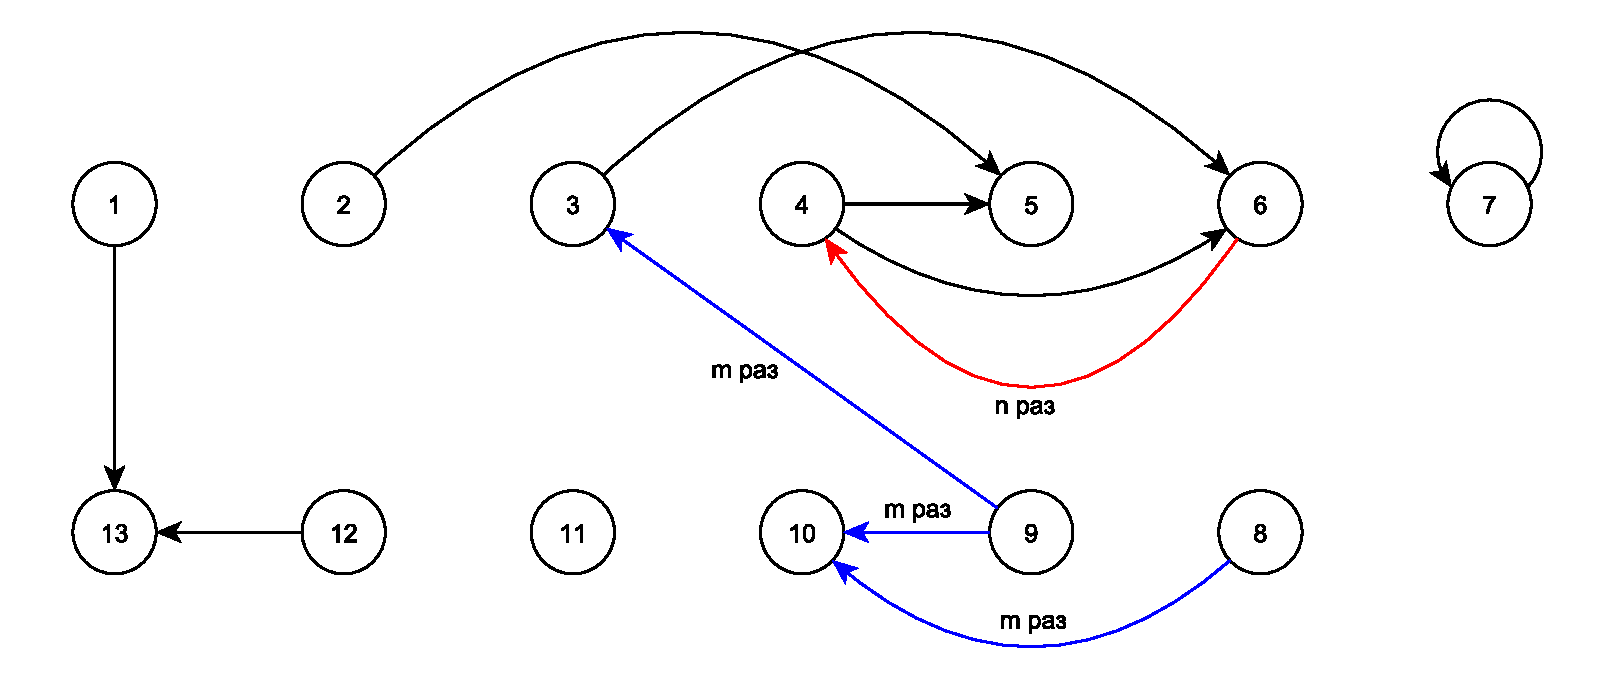
\includegraphics[height=0.27\textheight]{images/ИИ.pdf}
	\caption{Информационная история}
	\label{fg:ii}
\end{figure}

Причины, по которым вершина 7 обращается сама к себе, а вершина 11 не связана ни с какой другой, описаны в разделе информационного графа.

\section*{Возможность распараллеливания}
Распараллеливание алгоритма поиска подстроки в строке (файле) заключается в разделении его на несколько частей и обработке каждой части отдельным потоком.